\documentclass{beamer}
\usepackage{kotex}
\usepackage[utf8]{inputenc}
\usepackage[T1]{fontenc}
\usepackage{setspace}
\usepackage{color}
\usepackage{listings}
\usepackage{mathtools}
\usepackage{physics}
\usepackage[variablett]{lmodern}
\usetheme{berlin}
\title{\TeX\ 사용의 입문}
\author{신주형}
\institute{Sejong Academy of Science and Arts}
\usecolortheme{beaver}
\setbeamertemplate{itemize items}[square]
\setbeamertemplate{itemize subitem}[triangle]

\lstset{language=tex, tabsize=2, extendedchars=true,texcl=true,stringstyle=\color{black!50}\ttfamily,basicstyle=\small\sffamily,numbers=left,numberstyle=\tiny,frame=tb,columns=fullflexible,showstringspaces=false}

\newcommand{\sourcecode}[4]
{\begin{frame}
	\frametitle{Source Code}
	
	\begin{columns}[T]
		\begin{column}{.5\textwidth}
			\begin{center}
				\includegraphics[#4]{#1}
			\end{center}
		\end{column}
		\begin{column}{.5\textwidth}
			\begin{center}
				\begin{lstinputlisting}[#3,frame=single]{#2}
				\end{lstinputlisting}
			\end{center}
		\end{column}
	\end{columns}
\end{frame}}


\begin{document}
	\begin{frame}
		\maketitle
	\end{frame}
\section{\TeX?}
	\begin{frame}{What is \TeX?}
	\begin{itemize}
		\item{Donald Knuth가 만든 문서 조판 언어.}
		\item{WYSIWYG 방식의 워드 프로세서가 아님.}
		\item{명령어를 치고 컴파일하면 예쁘게 조판해 주는 형식.}
	\end{itemize}
	\end{frame}
	\begin{frame}{Why \TeX \ is Good?}
	\begin{itemize}
		
		\item{수식 환경의 간편함}
		\item{문서의 질이 상승}
		\item{생각보다는 간편하다.}
		\begin{itemize}
			\item{매크로의 활용}
			\item{패키지의 활용}
			\item{문서 양식의 활용(Internet에서 get)}
			\begin{itemize}
				\item{ktug wiki에 자세한 내용이 있다.}
				\item{google에 물어봐도 자세한 내용이 있다.}
				\item{그 외의 세부적 내용은 해당 패키지의 도움말을 찾아볼 것.}
			\end{itemize}
		\end{itemize}
	\end{itemize}
	\end{frame}
	\begin{frame}{Why \TeX \ is Good?}
		\framesubtitle{다시 말하면요...}
		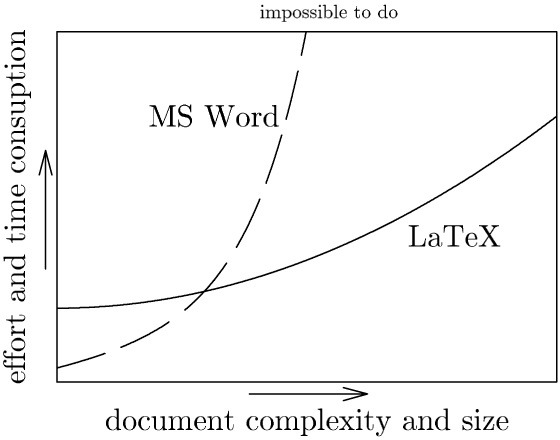
\includegraphics[scale=0.3]{ffjqm_img.jpg}\centering
	\end{frame}
	\begin{frame}{Starting \TeX}
	
	\begin{itemize}
		\item{프로그래밍의 요소가 섞여 있다는 것을 유념할 것.}
		\item{특히 \TeX 에서는 '환경' 개념이 아주 중요함}
		\begin{itemize}
			\item{환경이란 문서 내부에서 특징적으로 지정해주는 것을 의미\\ (ex: 수식 환경, 가운데 정렬 환경, $\cdots$)}
		\end{itemize}
	\end{itemize}
	\end{frame}

	\begin{frame}[fragile]
		\frametitle{\TeX \ 문서의 구조}
		\begin{enumerate}
			\item Preamble(전처리구): 문서의 설정, 양식, Package 등을 첨부
			\begin{itemize}
				\item \verb|\documentclass[10pt,a4papersize]{article}|:문서의 종류를 설정
				\item 
				\verb|\usepackage{tikz}|: Package 추가(\verb|#include <stdio.h>|)
				\item 기타 여러 가지가 있으나 (ex:\verb|\usecolortheme{beaver}|) 여기까지는 몰라도 됨 \ldots
			\end{itemize}
			\item Body(본문): 본문
		\end{enumerate}
		\begin{itemize}
			\item  전처리구를 깔끔히 한 파일로 만들고(즉, 문서 양식을 만들고) 본문은 \verb|\include{file}|을 통해 다른 파일에 쉽게 쓸 수 있다.(우리의 목표)
		\end{itemize}
	\end{frame}
\section{\TeX \ 입문하기 \ldots}
	\begin{frame}[fragile]
	\frametitle{문서 만들기}
	\framesubtitle{Hello World 쓰기}
		\begin{itemize}
			\item{목표: Hello World를 출력해보자.}
			\item{ Hint: 문서를 만들기 위해서는 \verb|\documentclass{...}|로 문서 종류를 정하고 문서 환경을 \verb|\begin{document} ... \end{document}|로 만들어야 함.}
		\end{itemize}
	\end{frame}

\sourcecode{ex1.jpg}{ex1.tex}{basicstyle=\ttfamily\small}{width=\linewidth}

\begin{frame}[fragile]
\frametitle{문서 만들기}
\framesubtitle{안녕하세요 쓰기}
\begin{itemize}
	\item{목표: 안녕하세요를 출력해보자.}
	\item{ Hint: 아까와 똑같이 하면$\cdots$ 될까?}
\end{itemize}
\end{frame}

\sourcecode{ex2.jpg}{ex2.tex}{basicstyle=\ttfamily\small}{width=\linewidth}

\begin{frame}[fragile]
\frametitle{문서 만들기}
\framesubtitle{안녕하세요 쓰기}
\begin{itemize}
	\item{\verb|\kotex| 패키지를 쓰면 한글을 쓸 수 있음.}
	\item{한글 전용 환경인 \verb|\oblivoir| 환경을 쓰는 것을 추천.}
\end{itemize}
\end{frame}

\sourcecode{ex3.jpg}{ex3.tex}{basicstyle=\ttfamily\small}{width=\linewidth}

\begin{frame}[fragile]
\frametitle{문서 만들기}
\framesubtitle{'큰' 안녕하세요 쓰기}
\begin{itemize}
	\item{목표: 아까보다 크기가 큰 안녕하세요를 출력해보자.}
	\item{ Hint: \verb|\large| 명령어를 사용해보자.}
\end{itemize}
\end{frame}

\sourcecode{ex4.jpg}{ex4.tex}{basicstyle=\ttfamily\small}{width=\linewidth}

\begin{frame}[fragile]
\frametitle{문서 만들기}
\framesubtitle{'큰' 안녕하세요 쓰기}
\begin{itemize}
	\item{\TeX 에서는 폰트 크기 변경이 자유롭지는 않음.}
	\item{문서를 결정할 때 기본 폰트 크기를 같이 결정할 수 있음 (\verb|\documentclass[12pt]{oblivoir}|)}
	\begin{itemize}
		\item{단, 10pt, 11pt, 12pt만 가능함.}
	\end{itemize}
\end{itemize}
\end{frame}

\begin{frame}[fragile]
\frametitle{문서 만들기}
\framesubtitle{노래 가사 쓰기}
\begin{itemize}
	\item{다음을 써 보자.}
	\begin{columns}[T]
	\begin{column}{.5\textwidth}
	\begin{itemize}
		\item{
		바보야 오늘은\\
		안된다고 말하지마\\
		오늘만큼은 내게도\\
		꼭 기회를 줘\\
		사랑스럽게 웃는 것도\\
		예쁘게 말하는 것도\\
		많이 연습했어\\
		보고 싶어도 참으라고 하지 마
		}
	\end{itemize}
	\end{column}
	\begin{column}{.5\textwidth}
	\begin{itemize}
		\item{
		(다음 문단)\\
		Baby 난 좀 억지 부리는 것도 맞아\\
		오늘도 내 눈물 연기로\\
		받아낸 너와의 데이트\\
		보고 싶어도\\
		매일 꾹 참고 있어도\\
		나는 네가 안아주기만 하면\\
		사르르르르 녹아 Yeah
		}
	\end{itemize}
	\end{column}
	\end{columns}
\end{itemize}
\end{frame}

\begin{frame}
\frametitle{문서 만들기}
\framesubtitle{노래 가사 쓰기}
\begin{columns}
	\begin{column}{.5\textwidth}
		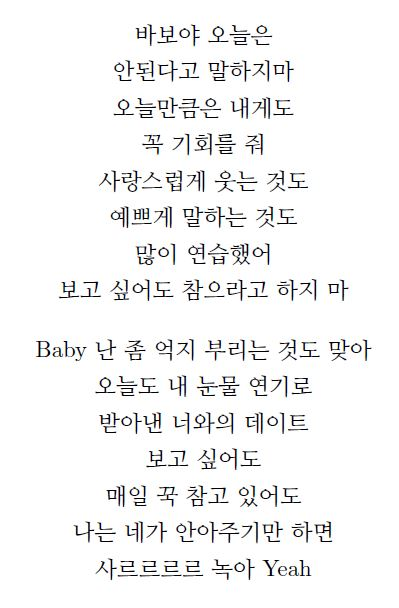
\includegraphics[scale=0.5]{ex5.jpg}
	\end{column}
	\begin{column}{.5\textwidth}
		\begin{itemize}
			\item{결과적으로 우리는 이런 형태의 글을 쓰기를 원한다.}
			\item{일단 한 번 시도해보자.}
		\end{itemize}
		
	\end{column}
\end{columns}
	
\end{frame}

\sourcecode{ex5-1.jpg}{ex5-1.tex}{basicstyle=\ttfamily\tiny}{width=\linewidth}

\begin{frame}
\frametitle{문서 만들기}
\framesubtitle{노래 가사 쓰기-해결1}
	\begin{itemize}
		\item{안타깝게도, 엔터 한 번으로는 줄바꿈이 되지 않음.}
		\item{엔터 두 번이면 새로운 문단으로 인정하기 때문에 우리가 원하는 띄어쓰기와는 다름.}
		\item{엔터 세 번부터는 엔터 두 번과 같은 효과}
		\item{어떻게 하면 좋을까?}
	\end{itemize}
\end{frame}

\begin{frame}[fragile]
\frametitle{문서 만들기}
\framesubtitle{노래 가사 쓰기-해결1}
	\begin{itemize}
		\item{\TeX 에는 강제 줄바꿈 명령어가 있다.}
		\item{\verb|\\|와 \verb|\newline|이 그것}
		\begin{itemize}
			\item{\verb|\newline|은 진짜로 '강제' 줄바꿈이다.}
			\item{\verb|\\|를 이용하자.}
		\end{itemize}
	\end{itemize}
\end{frame}

\sourcecode{ex5-2.jpg}{ex5-2.tex}{basicstyle=\ttfamily\tiny}{width=\linewidth}

\begin{frame}[fragile]
\frametitle{문서 만들기}
\framesubtitle{노래 가사 쓰기-해결2}
\begin{itemize}
	\item{\TeX 에서는 문단을 만들 때마다 들여쓰기를 실행}
	\item{\verb|\noindent|명령어를 통해 이를 제거 가능}
	\end{itemize}
\end{frame}

\sourcecode{ex5-3.jpg}{ex5-3.tex}{basicstyle=\ttfamily\tiny}{width=\linewidth}

\begin{frame}[fragile]
\frametitle{문서 만들기}
\framesubtitle{노래 가사 쓰기-해결3}
\begin{itemize}
	\item{가운데 정렬을 하고 싶다.}
	\item{\verb|\begin{center}...\end{center}|명령을 이용하자.}
\end{itemize}
\end{frame}

\sourcecode{ex5.jpg}{ex5.tex}{basicstyle=\ttfamily\tiny}{scale=0.4}

\begin{frame}[fragile]
\frametitle{문서 만들기}
\framesubtitle{노래 가사 쓰기-정리}
\begin{itemize}
	\item{\TeX 에서는 두 개 이상의 엔터를 문단 변화로 인식.}
	\item{강제 줄 이동은 \verb|\\|나 \verb|\newline|으로}
	\item{\verb|\noindent|를 통해 문단의 들여쓰기를 제거할 수 있음.}
	\item{\verb|\begin{center}...\end{center}|로 가운데 정렬 가능}
	\begin{itemize}
		\item{오른쪽 정렬은 \verb|\begin{flushright}...\end{flushright}|}
		\item{왼쪽 정렬은 \verb|\begin{flushleft}...\end{flushleft}|}
	\end{itemize}
	\item{\verb|\vspace{length}|를 통해 줄 간격을 만들 수 있음}
	\begin{itemize}
		\item{칸 사이의 간격은 \verb|\,|, \verb|\;|, \verb|\quad|, \verb|\qquad|등으로 만들 수 있음(꼼수다!)}
		\item{띄어쓰기 한 칸은 \verb|\ |로 해결 가능.}
		\item{그 외는 \verb|\phantom{ }| 명령어나 \verb|\hspace{10pt}|로 띄어쓰기를 하자.}
	\end{itemize}
\end{itemize}
\end{frame}
\section{수식하기}
\begin{frame}[fragile]
	\frametitle{제목 만들기}
	\begin{itemize}
		\item{목표: 제목은 \TeX \, is SO Easy, 이름은 모두의 \TeX \, 동아리로 제목을 만들어 보자.}
		\item{Hint: 아까 배운 것들을 활용하여 만들 수 있다. (\TeX 은 \verb|\TeX|으로 조판할 수 있는데, 이런 특수 문자 뒤의 띄어쓰기는 무시된다. 강제로 칸 사이 간격을 만들어야 할 것이다.)}
	\end{itemize}
\end{frame}

\sourcecode{ex6.jpg}{ex6.tex}{basicstyle=\ttfamily\tiny}{width=\linewidth}

\begin{frame}[fragile]
\frametitle{제목 만들기}
\begin{itemize}
	\item{가운데 정렬 환경을 통해 제목을 만들 수 있음.}
	\item{\verb|\maketitle|을 통해 편하게 제목을 만들 수 있음.}
\end{itemize}
\end{frame}

\sourcecode{ex6-1.jpg}{ex6-1.tex}{basicstyle=\ttfamily\tiny}{width=\linewidth}

\begin{frame}[fragile]
\frametitle{강조하기}
\begin{itemize}
	\item{목표: 내용을 \textbf{이렇게}, \textit{이렇게},\\ \emph{이렇게}, \underline{이렇게}, \dotemph{이렇게} 강조해보자.}
	\item{Hint: 각각 \verb|\textbf{...}|, \verb|\textit{...}|, \verb|\emph{...}|, \verb|\underline{...}|, \verb|\dotemph{...}|로 표현할 수 있다.}
\end{itemize}
\end{frame}

\sourcecode{ex12.jpg}{ex12.tex}{basicstyle=\ttfamily\tiny}{width=\linewidth}

\begin{frame}[fragile]
	\frametitle{강조하기}
	\begin{itemize}
		\item{\verb|\textbf{...}|, \verb|\textit{...}|등은 폰트를 바꾸는 것이고, \verb|\emph{...}|는 상황에 맞춰 단어를 강조함.}
		\item{oblivoir에서는 \verb|\textit{한국어}|가 잘 적용되지 않음.}
		\item{oblivoir를 사용하면 \verb|\dotemph{...}|으로 단어를 강조할 수 있음.}
	\end{itemize}
\end{frame}
\section{`수식'하기}
\begin{frame}[fragile]
\frametitle{수식 만들기}
\framesubtitle{수식 환경 사용하기}
\begin{itemize}
	\item{\TeX 에서는 수식 환경이라는 특별한 환경이 존재}
	\item{목표: 수식 환경을 이용해서 근의 공식($x=\frac{-b\pm\sqrt{b^2-4ac}}{2a}$)를 써 보자.}
	\item{Hint:\verb|\begin{eqaution}...\end{eqaution}|을 이용해보자.}
	\item{Hint: 분수는 \verb|\frac{분자}{분모}|로, 루트 기호는 \verb|\frac{...}|으로 쓸 수 있다. $\pm$ 기호는 \verb|\pm|으로 쓴다.}
\end{itemize}
\end{frame}

\sourcecode{ex7.jpg}{ex7.tex}{basicstyle=\ttfamily\tiny}{width=\linewidth}

\begin{frame}[fragile]
\frametitle{수식 만들기}
\framesubtitle{수식 환경 사용하기}
	\begin{itemize}
		\item{\verb|\begin{eqaution}...\end{eqaution}|은 우리를 수식 환경의 세계로 인도함.}
		\item{equation 환경은 수식을 하나밖에 적을 수 없고, 뒤에 수식 번호가 적혀 나옴.}
	\end{itemize}
\end{frame}

\begin{frame}[fragile]
\frametitle{수식 만들기}
\framesubtitle{수식 참조하기}
\begin{itemize}
	\item{목표: 아까 쓴 근의 공식 아래에 '식 (공식 번호)는 근의 공식이다'라고 써 보자.}
\end{itemize}
\end{frame}

\sourcecode{ex8.jpg}{ex8.tex}{basicstyle=\ttfamily\tiny}{width=\linewidth}

\begin{frame}[fragile]
\frametitle{수식 만들기}
\framesubtitle{수식 참조하기}
\begin{itemize}
	\item{\verb|\label{key}|와 \verb|\ref{key}|를 통해 수식 참조 가능}
	\item{수식 번호를 삭제하고 싶으면 \verb|\nonumber| 명령어 사용.}
	
	\item{\verb|\(...\)|는 수식 번호가 없는 행 내 수식을 만들고, \verb|\[...\]|는 수식 번호가 없는 표시형 수식을 만든다.}
\end{itemize}
\end{frame}

\begin{frame}[fragile]
\frametitle{수식 만들기}
\framesubtitle{여러 개의 수식 쓰기(I)}
\begin{itemize}
	\item{다음을 써 보자.}
	\item{\begin{equation}
		\begin{gathered}
		\alpha + \beta = -\frac{b}{a}\\
		\alpha\beta = \frac{c}{a}
		\end{gathered}
	\end{equation}}
	\item{Hint:\verb|\usepackage{mathtools}|를 넣고, \verb|\begin{equation} \begin{gathered}...|
	\verb|\end{gathered} \end{equation}|로 식을 삽입하자.}
\end{itemize}
\end{frame}

\sourcecode{ex9.jpg}{ex9.tex}{basicstyle=\ttfamily\tiny}{width=\linewidth}

\begin{frame}[fragile]
\frametitle{수식 만들기}
\framesubtitle{여러 개의 수식 쓰기(II)}
	\begin{itemize}
		\item{다음을 써 보자.}
		\item{\tiny \begin{align}
				1+2+3+\cdots+n &= \sum_{k=1}^{n}k \nonumber\\
				&= \frac{1}{2}\sum_{k=1}^{n} (k+(n+1-k)) \nonumber\\
				&= \frac{1}{2}\sum_{k=1}^{n} (n+1) \nonumber\\
				&= \frac{n(n+1)}{2}
		\end{align}}
		\item{Hint:$\cdots$는 \verb|\cdots|으로 만들고, $\sum_{k=1}^{n}k$는 \verb|\sum_{k=1}^{n}k|로 만든다.}
	\end{itemize}	
\end{frame}

\sourcecode{ex10.jpg}{ex10.tex}{basicstyle=\ttfamily\tiny}{width=\linewidth}

\begin{frame}[fragile]
\frametitle{수식 만들기}
\framesubtitle{여러 개의 수식 쓰기(II)}
\begin{itemize}
	\item{\verb|\usepackage{mathtools}|을 첨부하고 \verb|\begin{align}...\end{align}|}을 이용하면 \verb|...&=...\\...&=...|을 통해 묶어줄 위치를 선정할 수 있음.
\end{itemize}	
\end{frame}

\begin{frame}[fragile]
\frametitle{수식 만들기}
\framesubtitle{글 안에 수식 넣기}
\begin{itemize}
	\item{다음을 써 보자.}
	\item{물체의 변위를 $\vec{x}$라고 한다면 $\dv[2]{\vec{x}}{t}$는 가속도를 의미하게 된다. 이 때 $\vec{F}_{net}=m\dv[2]{\vec{x}}{t}$가 성립한다.}
	\item{Hint: \verb|$...$|로 수식 환경을 글 안에서 만들 수 있다. 벡터 표시는 \verb|\vec{a}|로 구현할 수 있다.}
\end{itemize}	
\end{frame}

\sourcecode{ex11.jpg}{ex11.tex}{basicstyle=\ttfamily\tiny}{width=\linewidth}

\begin{frame}[fragile]
\frametitle{수식 만들기}
\framesubtitle{글 안에 수식 넣기}
\begin{itemize}
	\item{글 안의 수식은 \verb|$...$|를 통해 넣을 수 있음.}
	\item{\verb|\usepackage{physics}|를 이용해 미분을 더 편하게 사용할 수 있음.}
\end{itemize}
\end{frame}

\begin{frame}[fragile]
\frametitle{수식 만들기}
\framesubtitle{기타 수식에 관한 정보}
	\begin{itemize}
		\item{만약 수식 번호를 붙이지 않는 환경을 쓰고 싶으면 \verb|align*|,\verb|gather*|등 뒤에 *을 붙이면 됨.}
		\item{기타 수식 기호들}
		\begin{itemize}
			\item{\verb|\sqrt[root]{arg}|:제곱근 기호}
			\item{\verb|\int_{text}^{max}|:적분 기호}
			\item{\verb|\delta|, \verb|\Delta|:그리스 문자}
			\item{\verb|a^{n}|, \verb|a_{n}|:위 첨자, 아랫 첨자}
			\item{\verb|\begin{cases} ... \end{cases}|: 중괄호로 경우 나누기}
			\item{\verb|\left( ... \right)|: 수식 크기에 맞는 괄호 제작}
			\item{기타 기호들은 \TeX Studio의 편집창 옆의 바에서 쉽게 삽입할 수 있음}
		\end{itemize}
	\end{itemize}
\end{frame}

\begin{frame}
\frametitle{수식 만들기}
\framesubtitle{examples}
	\begin{gather*}
		\begin{cases}
		f(x)=\int_{-\infty}^{\infty}g(\alpha)e^{i\alpha x}d\alpha,\\
		g(\alpha)=\frac{1}{2\pi}\int_{-\infty}^{\infty}f(x)e^{-i\alpha x}dx
		\end{cases}\\ \\
		i\hbar\pdv{\Psi}{t}=\left[-\frac{\hbar^2}{2m}\laplacian+V\right]\Psi
	\end{gather*}
\end{frame}
\begin{frame}[fragile]

\section{정리}
\frametitle{마치며}
\begin{itemize}
	\item{지금 배운 게 \TeX 의 빙산의 일각이라는 사실.}
	\begin{itemize}
		\item{그림 첨부, 벡터 그래픽, 매크로, 등등 아직 해야 할 것들이 많다\ldots}
	\end{itemize}
	\item{그러나 이만큼으로도 내가 원하는 문서의 90\%는 만들 수 있다.}
	\begin{itemize}
		\item{나머지 10\%는 인터넷에 검색해서 배우도록 하자.}
	\end{itemize}
	\item{142분 동안 익히는 \LaTeX \phantom{ } 2$\epsilon$에 설명이 잘 되어 있다. 추가로 찾아볼 것.}
\end{itemize}
\end{frame}

\section{Additional \TeX?}
\begin{frame}
\frametitle{남은 10\%에 관한 설명}
\begin{itemize}
	\item 남은 10\%는 심하면 문서에서 사용하지 않을 가능성도 크다.
	\item 그럼에도 이런 것이 있다- 정도를 보여주기 위해 다음을 소개할 예정.
	\begin{itemize}
		\item tabular, minipage, etc(문서 분할하기)
		\item 이미지 추가
		\item 벡터 그래픽 제작
		\item 매크로 지정
	\end{itemize}
\end{itemize}
\end{frame}

\begin{frame}
\frametitle{tabluar 환경}
\begin{itemize}
	\item 다음의 표를 만들어보자.
	\item \begin{tabular}{c|c|c}
		\multicolumn{1}{c}{} & \TeX & MS Word \\
		\hline\hline
		Difficulty & Hard & Easy\\
		\hline
		Type & WYSIWYM & WYSIWYG \\
		\hline
		Easy Document & \multicolumn{2}{c}{Easy}\\
		\hline
		Hard Document & Easy & Hard
	\end{tabular}
\end{itemize}


\end{frame}

\sourcecode{ex13.jpg}{ex13.tex}{basicstyle=\ttfamily\tiny}{width=\linewidth}

\begin{frame}
\frametitle{tabluar 환경}
	\begin{itemize}
		\item{tabular 환경은 표를 제작해줌.}
		\item{수식의 경우 array 환경을 사용(matrix 환경도 존재.)}
	\end{itemize}
\end{frame}

\begin{frame}[fragile]
\frametitle{minipage 환경}
\begin{itemize}
	\item 문서를 절반으로 쪼개서 각각 글을 채워 넣자.
	\item 다양한 명령어가 존재 (\verb|box|류 명령어, \verb|minipage|, \verb|\begin{multicol}...\end{multicol}|(\verb|\usepackage{multicol}|))등이 존재
\end{itemize}
\end{frame}

\sourcecode{ex14.pdf}{ex14.tex}{basicstyle=\ttfamily\Tiny}{width=\linewidth}

\begin{frame}[fragile]
\frametitle{minipage 환경}
\begin{itemize}
	\item \verb|\framebox[width]{text}|이외에도 \verb|\colorbox|, \verb|\shadowbox|, \verb|\doublebox|(\verb|fancybox|패키지 필요) 등을 사용할 수 있음.
	\item \verb|minipage|환경은 \verb|\parbox{width}{text}|와 비슷한 효과(문서 안의 박스를 설정)
	\item 자세한 이론은 우선 생략.
\end{itemize}
\end{frame}

\begin{frame}
\frametitle{이미지 추가}
\begin{itemize}
	\item 이미지를 하나 추가해보자.
\end{itemize}
\end{frame}

\sourcecode{ex15.jpg}{ex15.tex}{basicstyle=\ttfamily\tiny}{scale=0.5}

\begin{frame}
\frametitle{이미지 추가}
\begin{itemize}
	\item graphics나 graphicx 패키지를 이용해 그래픽을 문서 안에 추가할 수 있음.
	\item figure 환경 안에 그림을 첨부하고 caption을 달 수 있다.
	\item 문서랑 어울리게 하는 것이 어려움. (minipage를 열심히 이용하거나, kswrapfig 패키지를 이용하여 할 수 있음)
\end{itemize}
\end{frame}

\begin{frame}
\frametitle{벡터 그래픽 제작}
\begin{itemize}
	\item 물리 문제에 사용할 진자 그림을 그려보자.
	\item tikz 패키지를 이용해 벡터 그래픽을 직접 만들 수 있음.
\end{itemize}

\end{frame}

\sourcecode{ex16.pdf}{ex16.tex}{basicstyle=\ttfamily\TINY}{width=\linewidth}

\begin{frame}
\frametitle{벡터 그래픽 제작}
\begin{itemize}
	\item Tikz 패키지 말고 PSTricks도 많이 유명함.(둘 다 배우는 것은 비추)
	\item 그림 그릴 때는 standalone 환경에서 작업하는 것도 좋다.
	\item 사실 좀 어려움\ldots
	\begin{itemize}
		\item Ipe, TikzEdit 등 벡터 그래픽 편집 프로그램을 사용하면 조금 쉬워진다.
		\item 지오지브라에도 벡터 그래픽 제작 매크로가 존재한다.
		\item 가끔은 그림판과 타협하는 것이 더 좋을지도 모른다.
	\end{itemize}
\end{itemize}
\end{frame}

\begin{frame}
\frametitle{매크로 지정}
\begin{itemize}
	\item \TeX 에는 매크로 기능이 존재(아마 프로그래밍으로서의 \TeX 을 가장 잘 드러내는 부분)
	\item 매크로를 사용하여 항등행렬을 간단히 출력해보자.
\end{itemize}
\end{frame}

\sourcecode{ex18.jpg}{ex18.tex}{basicstyle=\ttfamily\Tiny}{scale=0.5}

\begin{frame}[fragile]
\frametitle{매크로 지정}
\begin{itemize}
	\item 새로운 명령어를 지정하는 것은 \verb|\newcommand{cmd}{def}|,\verb|\def|,
	\verb|\newenvironment{text}{begdef}{enddef}|등이 존재
	\item 다만 C처럼 함수를 만든다고 생각하면 조금 곤란함(가능은 하다만\ldots)
	\item 알아두면 글 작업이 편리해짐.(특히 이미지 첨부, 벡터 그래픽 제작에서)
\end{itemize}
\end{frame}
\end{document}